\scanpage{8}

\uline{Corollary.} This open set is dense if and only if for \unsure{every|every} \uline{maximal} point $x\in X$, $\underline O_{X,x}$ is reduced and $k(x)$ is a \uline{separable} extension of $k$ $[\Leftrightarrow$ \inserted{\unsure{in case an|in the case of an} extension of finite type} étale extension of a purely \unsure{transcendental|transcendental|transcendental or} extension$]$

\uline{Corollary} If $k$ is perfect, the set of points where $X$ is smooth is a dense open set.

\uline{NB} We have an analogous \unsure{result|result} for \uline{geometric normality}, without a finiteness condition. If $X$ is \deleted{\unsure{geometrically normal|geometrically normal}} \inserted{locally of} finite type over $k$, the set of points where $X$ is geometrically normal over $k$ is open, \inserted{and dense if $k$ is perfect} [An extension of a field is geometrically normal if and only if it is separable)

\figure{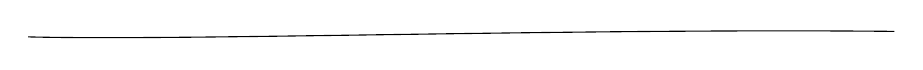
\begin{tikzpicture}\draw (0,0) .. controls (2,-.05) and (7,.11) .. (11,.07);\end{tikzpicture}}

\uline{Proposition} $G$ group over field $k$. Equivalent conditions

\margin{also works if $X$ a \deleted{\unsure{group|space}} \inserted{scheme} on which $G$ acts and such that \deleted{$G\times X\xrightarrow{\unsure{\pi|p}} X$} $G\times X\longrightarrow X\times X$ surjective $(g,x)\longmapsto(gx,x)$ ($X$ essentially homogeneous)}% slanted

a) $G$ \deleted{\unsure{geometrically normal|geometrically normal}} separable $/k$ at a point \qquad a$'$) $G$ separable $/k$ \deleted{at a point}

b) $G$ geometrically normal over $k$

c) (If $G$ locally of finite type over $k$) $G$ smooth $/k$

We obviously have \inserted{c $\Rightarrow$} b) $\Rightarrow$ a$'$) $\Longrightarrow$ a) \deleted{$\Longrightarrow$ \unsure{b)|b)?}}.

\margin{\uline{NB} If $G$ of finite type over $k$, then $G$ \deleted{\unsure{re|ré}} \unsure{reduced|reduced} $\Rightarrow G$ separable? \deleted{(\unsure{is it that|and if not|is it} the \unsure{$k$|$h$} \unsure{is} \unsure{stable in|being given}}}% slanted

a) $\Rightarrow$ b) \qquad Let $g\in G$, \deleted{a} maximal point of $G$. \deleted{\unsure{geometric|generic}} \deleted{for $g$ \unsure{$G$ is geometrically normal at $g$|to be geometric it suffices that $g$},} Then $k(g)$ is a separable extension of $k$, so $G$ is geometrically normal at $g$. \deleted{Thus, at the cost \unsure{of making an extension|of an extension} by descent we are reduced to \unsure{considering the case|considering the assertion} for $g$ rational over $k$.} \deleted{Let $g'$ be a maximal point of $G$, we know that $G$ is geometrically normal at $g'$; making an extension} Thus $G$ has \uline{a} point $g$ where it is geometrically normal. Let us prove that the same holds for every other point $g'$. By extension of the base, we are reduced to the case where $g$, $g'$ rational over $k$. But then they are conjugate by translation !

b) $\Rightarrow$ a) \qquad \unsure{Esq.|Est.} in proof.

\uline{Corollary 1} Let $k$ be perfect. Then $G_{\text{\unsure{red|réd}}}$ is geometrically normal \unsure{$\bar k$|$k$|$\bar B$} (resp. smooth, if $G$ is locally of finite type over $k$)

% archive sheet number: 7
